%
% char.tex -- characteristics in problem 30000016
%
% (c) 2018 Prof Dr Andreas Müller, Hochschule Rapperswil
%
\documentclass[tikz]{standalone}
\usepackage{amsmath}
\usepackage{times}
\usepackage{txfonts}
\usepackage[utf8]{inputenc}
\usepackage{graphics}
\usepackage{ifthen}
\usepackage{color}
\usetikzlibrary{arrows,intersections}

\begin{document}
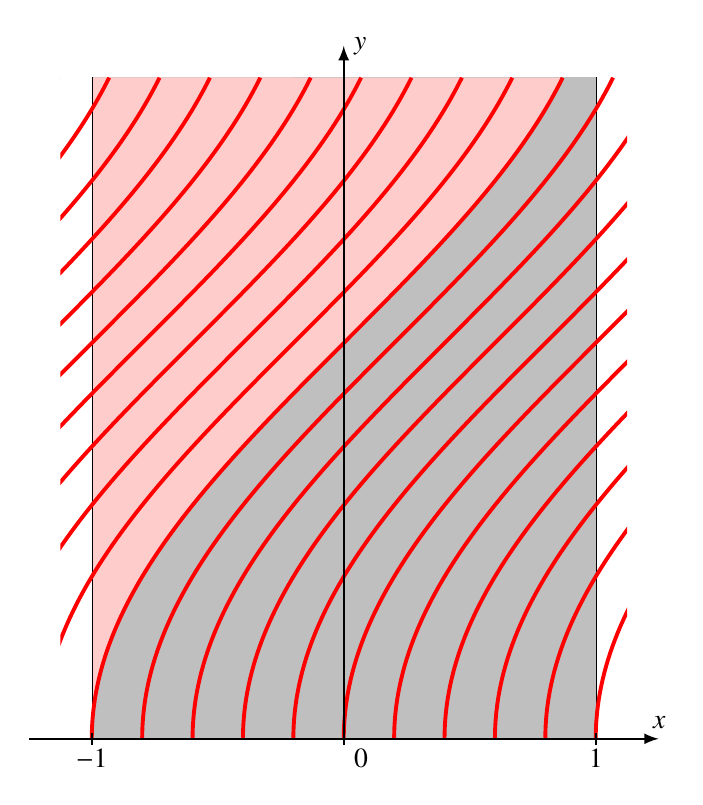
\begin{tikzpicture}[>=latex,thick,scale=0.8]
\fill[color=gray!50] (-4,0) rectangle (4,10.5);
\fill[color=red!20]
plot[domain=0:{10.5/4},samples=100] ({4*(-cos(180 * \x / (3.1415)))},{4*\x})
--(-4,10.5)--(-4,0)--cycle;
\draw[line width=0.1pt] (-4,0)--(-4,10.5);
\draw[line width=0.1pt] (+4,0)--(+4,10.5);
\begin{scope}

\clip (-4.5,0) rectangle (4.5,10.5);
\foreach \xnull in {-2,-1.8,...,3}{
\draw[color=red,line width=1.4pt] plot[domain=0:{10.5/4},samples=100] ({4*(\xnull - cos(180 * \x / (3.1415)))},{4*\x});
}
\end{scope}
\draw[->] (-5,0)--(5,0) coordinate[label=$x$];
\draw[->] (0,-0.1)--(0,11) coordinate[label={right:$y$}];
\draw (-4,-0.1)--(-4,0.1);
\draw (4,-0.1)--(4,0.1);
\node at (-4,0) [below] {$-1$};
\node at (4,0) [below] {$1$};
\node at (0,0) [below right] {$0$};
\end{tikzpicture}
\end{document}
